\chapter{Revisão da Literatura}
\label{chap:revisao-da-literatura}
\section{Ondas Gravitacionais}
\label{sec:ondas-gravitacionais}
\subsection{Introdução}
\label{subsec:ondas-gravitacionais:introducao}

Qualquer objeto com massa exerce uma força de atração sobre outros objetos com massa, conhecida como “gravidade”. De acordo com a teoria da gravidade de Sir Isaac Newton \cite{newton1687philosophiae}, quaisquer dois objetos exercem uma atração gravitacional um sobre o outro de igual valor e sentido oposto, quando uma massa muda de posição, todo o campo gravitacional em todo o universo muda instantaneamente, e as forças gravitacionais resultantes são instantaneamente alteradas de acordo.

Mas a Teoria da Relatividade Geral de Einstein \cite{albert1920realtivity}, afirma que nenhuma informação pode viajar mais rápido que a velocidade da luz, incluindo informações sobre as posições de massa no universo, que são comunicadas através do campo gravitacional. A Relatividade Geral prevê que uma mudança no campo gravitacional viajará pelo universo à velocidade da luz e são exatamente essas mudanças no campo gravitacional que são as ondas gravitacionais.

De forma geral, as ondas gravitacionais podem ser pensadas como as ondas criadas quando jogamos pedras na superfície de um lago. Essas ondas são perturbações na geometria do próprio espaço-tempo emitidas por colisões violentas que acontecem no universo, que se propagam à velocidade da luz, carregando informações sobre suas origens, bem como pistas sobre a natureza da própria gravidade \cite{LSC-VIRGO, abbott2016observation, ramos2018teoria}.

\begin{figure}[ht]
\centering
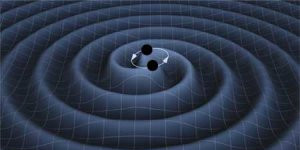
\includegraphics[width=.9\textwidth]{figuras/binary-wave_tn.jpg}
\caption{A impressão artística de ondas gravitacionais de dois buracos negros em órbita. [Imagem: T. Carnahan (NASA GSFC)]}
\label{fig:space-time}
\end{figure}

Ondas gravitacionais são criadas por massas móveis, da mesma forma que ondas eletromagnéticas são criadas por cargas em movimento. Mas como a gravidade é a mais fraca das quatro forças fundamentais (sendo as outras o eletromagnético, o nuclear fraco e o nuclear forte), as ondas gravitacionais são extremamente pequenas, produzindo um deslocamentos da ordem de \(10^{-18}\) metros, isto é, 1000 vezes menor que o diâmetro de um próton \cite{abbott2016observation}. Ondas dessa força serão produzidas por sistemas muito massivos que passam por grandes acelerações, como dois buracos negros em órbita que estão prestes a se fundir um com o outro. Como sistemas como esses são raros, essas fontes estarão a anos-luz de distância.

\subsection{Fontes e tipos de ondas gravitacionais}
\label{subsec:ondas-gravitacionais:fontes}

Em geral, qualquer aceleração que não seja esfericamente ou cilindricamente simétrica produzirá uma onda gravitacional \cite{abbott2017gw170814}. Considere uma estrela que vai se transformar em uma supernova, esta explosão produzirá ondas gravitacionais se a massa não for ejetada de maneira esférica simétrica, embora o centro de massa possa estar na mesma posição antes e depois da explosão. Outro exemplo é uma estrela em movimento. Uma estrela perfeitamente esférica não produzirá uma onda gravitacional, mas sim uma estrela irregular \cite{abbott2017gw170817}.

Com base nessas diferentes fontes, os cientistas do LIGO definiram quatro categorias de ondas gravitacionais: Ondas Gravitacionais Contínuas, Ondas Gravitacionais de Sistemas Binários, Ondas Gravitacionais Estocásticas e Ondas Gravitacionais de colapso gravitacional. Cada categoria gera um conjunto único de "impressões digitais" ou assinaturas vibracionais características que os interferômetros do LIGO podem detectar e que os pesquisadores podem procurar nos dados do LIGO \cite{Christensen_2018}.

Ondas gravitacionais contínuas são produzidas por sistemas que têm uma frequência razoavelmente constante e bem definida. Exemplos disso são sistemas de estrelas binárias ou de buracos negros orbitando um ao outro ou uma única estrela girando rapidamente em torno de seu eixo com uma grande inchaço ou outras imperfeições na sua forma esférica. Espera-se que estas fontes produzam ondas gravitacionais comparativamente fracas, uma vez que elas evoluem ao longo de períodos de tempo mais longos e são geralmente menos catastróficas do que as fontes que produzem ondas gravitacionais de sistemas binários ou de colapso gravitacional \cite{beheshtipour2020deep}, Figura~\ref{figondacontinua}.

\begin{figure}[ht]
\centering
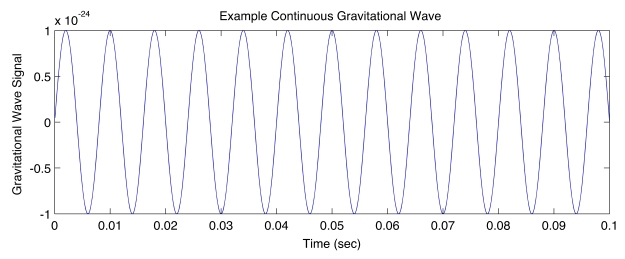
\includegraphics[width=.9\textwidth]{figuras/continuous_tn.jpg}
\caption{Um sinal de exemplo de uma fonte de onda gravitacional contínua. [Image: A. Stuver / LIGO]}
\label{figondacontinua}
\end{figure}

Ondas gravitacionais de sistemas binários são geradas durante o estágio final de vida de sistemas binários, onde os dois objetos se fundem em um. Esses sistemas são geralmente duas estrelas de nêutrons, dois buracos negros, ou uma estrela de nêutrons e um buraco negro cujas órbitas se degradaram até o ponto em que os dois objetos estão prestes a coalescer. À medida que os objetos giram em torno uma do outro, suas distâncias orbitais diminuem, retirando parte da energia orbital do sistema, enquanto suas velocidades aumentam \cite{Liu_2018}. Isso faz com que a frequência das ondas gravitacionais aumente até o momento da coalescência, Figura~\ref{figondainspiral}.

\begin{figure}[ht]
\centering
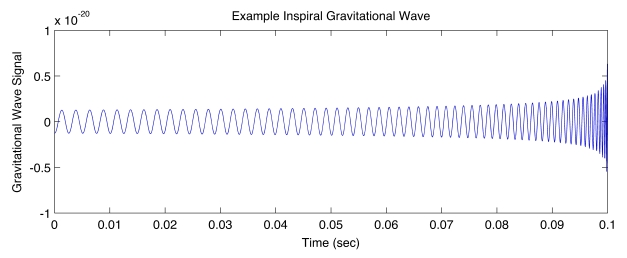
\includegraphics[width=.9\textwidth]{figuras/inspiral_tn.jpg}
\caption{Um sinal de exemplo de uma fonte de onda gravitacional de sistemas binários. [Image: A. Stuver / LIGO]}
\label{figondainspiral}
\end{figure}

As ondas gravitacionais de colapso gravitacional vêm de fontes desconhecidas ou imprevistas de curta duração. Há hipóteses de que alguns sistemas, como supernovas ou rajadas de raios gama, podem produzir ondas gravitacionais de colapso gravitacional, mas pouco se sabe sobre os detalhes desses sistemas para antecipar a forma que essas ondas terão \cite{Christensen_2018}, Figura~\ref{figondacolapso}.

\begin{figure}[ht]
\centering
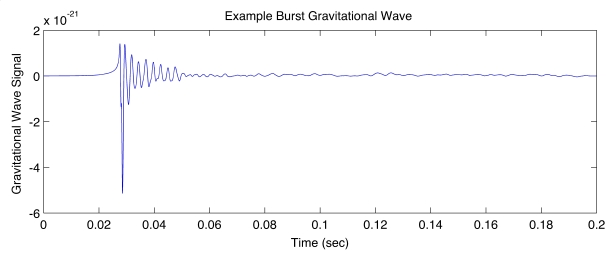
\includegraphics[width=.9\textwidth]{figuras/burst_tn.jpg}
\caption{Um sinal de exemplo de uma fonte de onda gravitacional de colapso. [Image: A. Stuver / LIGO usando dados de C. Ott, D. Burrows e outros]}
\label{figondacolapso}
\end{figure}

Ondas gravitacionais estocásticas são as ondas gravitacionais relíquias da evolução inicial do universo. Assim como radiação cósmica de fundo em micro-ondas(Cosmic Micro-wave Background - CMB), que provavelmente é a luz residual do Big Bang, essas ondas gravitacionais surgem de um grande número de eventos aleatórios e independentes combinados para criar um fundo de ondas gravitacionais cósmicas. Essas pequenas ondas de todas as direções compõem o que é chamado de sinal estocástico, tendo um padrão aleatório que pode ser analisado estatisticamente, mas não previsto com precisão \cite{Christensen_2018}.

Espera-se que o Big Bang seja o principal candidato para a produção dos muitos processos aleatórios necessários para gerar ondas gravitacionais estocásticas e, portanto, podem conter informações sobre a origem e a história do universo \cite{Christensen_2018}, Figura \ref{figondaestocastica}.

\begin{figure}[ht]
\centering
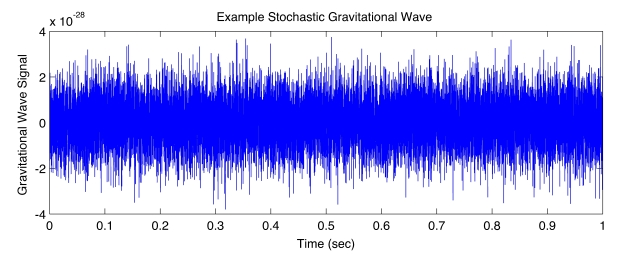
\includegraphics[width=.9\textwidth]{figuras/stochastic_tn.jpg}
\caption{Um sinal de exemplo de uma fonte de onda gravitacional estocástica. [Imagem: A. Stuver / LIGO]}
\label{figondaestocastica}
\end{figure}

\subsection{Equações de ondas Gravitacionais}
\label{subsec:ondas-gravitacionais:equacoes}

Uma maneira de se entender esse fenômeno matematicamente é através do cálculo que produz esse tipo de evento. Segundo a RG de Einstein, esses efeitos gravitacionais são descritos através da métrica $G_{\mu \nu}(x)$, que traz consigo informação acerca da curvatura do espaço-tempo.

Mas a equação de Einstein constitui um conjunto de 10 equações diferenciais parciais não lineares, o que, torna esse cálculo exaustivo e complexo. Uma maneira atrativa de se pensar nas equações de onda gravitacional produzidas por um sistema binário é tratar cada componente do sistema como um partícula. Segundo \cite{rubbo2007hands}, podemos fazer isto com a seguinte equação:

\begin{equation} \label{eqGW1}
\begin{split}
h(t) = \mathcal{A}(t)\cos \Phi(t),
\end{split}
\end{equation}

Na Equação \ref{eqGW1}, o $h(t)$ é a forma de onda gravitacional produzida pelos componentes(partículas) do sistema, também conhecida como deformação da onda gravitacional, $\mathcal{A}(t)$ é a amplitude dependente do tempo e $\Phi (t)$ é a fase da onda gravitacional. Ainda, segundo \cite{rubbo2007hands}, a amplitude $\mathcal{A}(t)$ pode ser expressa em termos dos parâmetros que caracterizam o sistema,

\begin{equation} \label{eqGW2}
\begin{split}
\mathcal{A}(t) = \frac{2(G\mathcal{M})^{5/3}}{c^4 r} \left(\frac{\pi}{P_{gw}(t)}\right)^{2/3} ,
\end{split}
\end{equation}
onde $G$ é a constante gravitacional de Newton, $c$ é a velocidade da luz, $r$ é a distância da luminosidade ao sistema binário e $P_{gw}(t)$ é o período da onda gravitacional. O valor $M \equiv (M_1 M_2)^{3/5}(M_1+M_2)^{-1/5}$ é a massa do \textit{chirp}\footnote{A massa do \textit{chirp} determina como o sistema evolui e o sinal de onda gravitacional emitido varia em amplitude e frequência, e é derivada da relação entre a massa total do sistema e a sua massa reduzida.} e comumente é usada na física das ondas gravitacionais, como uma escala de massa natural.

A fase das ondas gravitacionais, $\Phi (t)$, é análoga à fase para outro fenômeno das ondas, onde representa a localização do ciclo da onda que está colidindo com o detector no tempo $t$ e acompanha a evolução da amplitude da onda em função do tempo. A fase possui unidades de radianos e está relacionada à frequência da onda gravitacional $f_{gw}$ ou alternativamente ao período $P_{gw} = {f_{gw}^{-1}}$ pela integral da equação \ref{eqGW3}, onde, $\Phi_0$ é o valor da fase inicial, $\Phi_0=\Phi(t=0)$.

\begin{equation} \label{eqGW3}
\begin{split}
\Phi(t) = \Phi_0 + 2\pi \int_0^t \! \frac{{dt}^{'}}{P_{gw}(t^{'})}.
\end{split}
\end{equation}

Seguindo o exemplo dado em \cite{rubbo2007hands}, em que, os valores típicos da equação de amplitude de onda dado na Equação \ref{eqGW2}, foram substituídos por valores de um sistema binário de estrela de nêutrons localizado no centro de nossa galáxia, o mesmo afirma que as ondas gravitacionais são extremamente fracas e a amplitude de $\mathcal{A}$ é adimensional, portanto, a radiação gravitacional se manifesta na matéria ao induzir uma tensão. 

Em outros termos, a Equação \ref{eqGW1} proporciona a mudança relativa na distância entre dois pontos no espaço-tempo em função do tempo, tornando possível medir a separação entre duas massas e verificar se essas massas estão gerando uma onda gravitacional.

Como no eletromagnetismo, as ondas gravitacionais têm dois estados de polarização independentes designados por $\boldsymbol{+}$ e $\mathrm{X}$, como mostra a Figura \ref{figpolarization}. A polarização fornece, entre outras coisas, informação sobre a inclinação do plano orbital de um sistema binário em relação ao observador. Para um sistema binário, os dois estados são relacionados por uma mudança de fase de $90°$. Quando a linha de observação é paralela ao plano orbital do sistema, cada uma das componentes aparenta mover-se numa linha reta e neste caso possível, mostrar que a polarização das ondas gravitacionais emitidas será linear. 

\begin{figure}[ht]
\centering
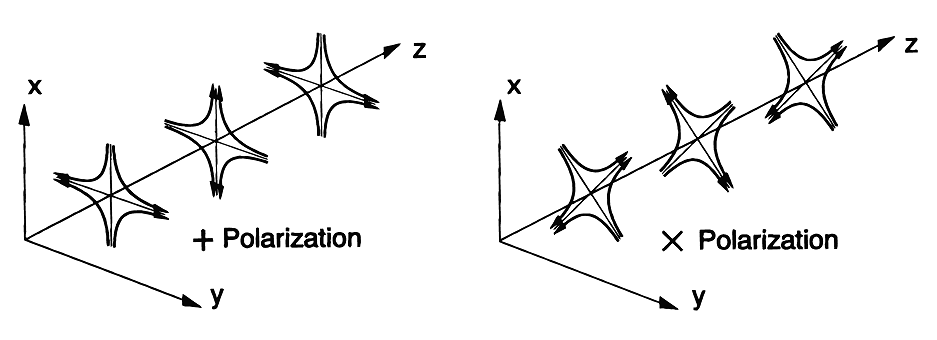
\includegraphics[width=.9\textwidth]{figuras/polarization.png}
\caption{Modos de polarização das ondas gravitacionais $\mathrm{h_{+}}$ e $\mathrm{h_{x}}$ propagando-se na direção $\mathrm{z}$. [Imagem: \cite{centrella2010black}]}
\label{figpolarization}
\end{figure}

Se, pelo contrário, a linha de observação for normal ao plano orbital, o movimento dos componentes será circular e a polarização observada será também circular. Entre estes dois casos limite existe uma gama de valores possível para a inclinação do plano orbital que pode em princípio ser deduzida através da polarização do sinal observado.

Consequentemente, a Equação \ref{eqGW1} captura a forma funcional dos dois estados de polarização. \cite{rubbo2007hands} afirma que ondas gravitacionais transportam energia e momento angular para longe do sistema binário, fazendo com que o período orbital diminua com o tempo, de acordo com

\begin{equation} \label{eqGW4}
\begin{split}
P_{orb}(t) = \left(P_0^{8/3} - \frac{8}{3}kt \right)^{3/8}
\end{split}
\end{equation}
onde $P_0$ é o período orbital no tempo $t = 0$, e $k$ é uma constante de evolução dada por:

\begin{equation} \label{eqGW5}
\begin{split}
k \equiv \frac{96}{5}(2\pi)^{8/3} \left(\frac{G\mathcal{M}}{c^3}\right)^{5/3}
\end{split}
\end{equation}

Como resultado do período orbital decrescente, os dois componentes binários se aproximaram lentamente, até o ponto em que colidem e coalesce em um único objeto remanescente, que ocorre quando $P_{orb}(t) = 0$.

Portanto, com a Equação \ref{eqGW1} é possível criarmos formas de ondas gravitacionais como mostra a Figura \ref{figmetade}. No entanto, é possível notar que a Equação \ref{eqGW1} não produz forma de onda, em que, o tempo é negativo, $P_{orb}(t) < 0$. Sendo assim, as formas de onda geradas por esse modelo não geram onda após a coalescência dos componentes. Devido a esta limitação este método de geração de ondas gravitacionais não será usado nesta pesquisa.

\begin{figure}[ht]
\centering
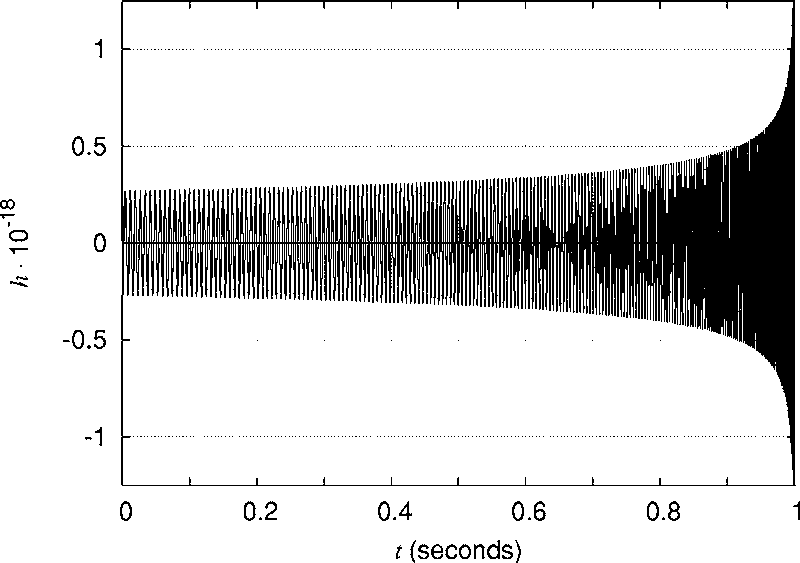
\includegraphics[width=.9\textwidth]{figuras/metade.png}
\caption{A forma de onda no último segundo antes da coalescência. Com a amplitude e a frequência do sinal aumentando com o tempo [Imagem: \cite{rubbo2007hands}]}
\label{figmetade}
\end{figure}

Esta é uma das maneiras que os astrônomos de ondas gravitacionais tem de extrair informações astrofísicas das formas de onda de sistemas binários observados. Claro que a análise de sinais reais é mais complexa. O principal desafio para a análise de dados reais é identificar o sinal oculto em um fluxo de dados com ruído. A abordagem mais comumente utilizada para esse problema na astronomia de ondas gravitacionais é usar a filtragem por coincidência. Se um sinal estiver presente em um fluxo de dados barulhento, o modelo fornecerá uma maneira de subtrair o ruído e deixar uma forma de onda limpa. Esta atividade assume que um modelo de sinal foi selecionado. Os astrônomos estimam os valores dos parâmetros astrofísicos que descrevem uma fonte de ondas gravitacionais a partir de formas de onda limpas \cite{rubbo2007hands}. 

\section{Redes Neurais Artificiais}
\label{sec:redes-neurais-artificiais}

\subsection{Introdução às Redes Neurais Artificiais}
\label{subsec:redes-neurais-artificiais:introducao}

Qualquer que seja o organismo multicelular, independente da sua complexidade e organização, possui algum tipo de sistema nervoso que é responsável por alimentar o organismo através de entradas sensoriais sobre informações do ambiente em que o organismo vive. As informações coletadas são processadas e comparadas com experiências passadas e posteriormente são transformadas em ações apropriadas para a situação ou absorvidas em forma de conhecimento \cite{haykin1994neural}.

Para o organismo complexo, humano, o neurônio biológico é basicamente o dispositivo computacional elementar do sistema nervoso que possui muitas entradas e uma saída. As entradas ocorrem através das conexões sinápticas, que conectam a árvore dendrítica aos axônios de outras células nervosas. Os sinais que chegam por estes axônios são pulsos elétricos conhecidos como impulsos nervosos ou potenciais de ação, constituindo a informação que o neurônio processará de alguma forma para produzir como saída um impulso nervoso no seu axônio \cite{kovacs1996redes}. 

O cérebro humano possui uma capacidade incrível de absorção de conhecimento e é considerado o processador mais fascinante que existente, podendo desempenhar funções como percepção, intuição, inferência, reconhecimento de padrões, controle motor, entre outros. Ele possui cerca de $10^{11}$ de neurônios e cada neurônio pode receber de 1.000 a 10.000 contatos sinápticos em seu corpo e dendritos, que são responsáveis por todas as funções e movimentos do nosso organismo. Os neurônios estão conectados uns aos outros através de sinapses, e juntos formam uma grande rede, denominada Rede Neural, que proporciona uma fabulosa capacidade de processamento e armazenamento de informação \cite{kovacs1996redes}, Figura~\ref{figneuronios}. 

\begin{figure}[ht]
\centering
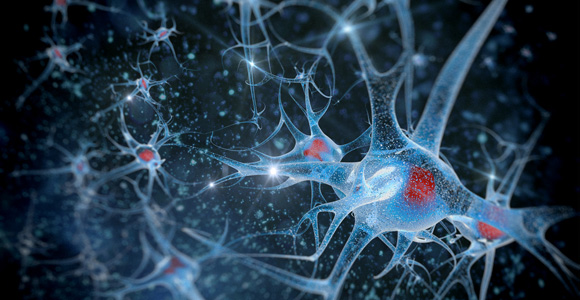
\includegraphics[width=1\textwidth]{figuras/axons.jpg}
\caption{Rede neural humana: o melhor processador de informações existente. [Imagem: \href{ https://neurogestion.wordpress.com}{ https://neurogestion.wordpress.com}]}
\label{figneuronios}
\end{figure}

\subsection{Redes Neurais Artificiais}
\label{subsec:redes-neurais-artificiais:rna}

Há algumas décadas, surgiu a ideia de modelar, computacionalmente, as conexões neurais do cérebro humano, buscando reproduzir as características do neurônio biológico. Neste contexto, as redes neurais artificiais foram desenvolvidas, tomando-se como base as redes de neurônios cerebrais e sinapses biológicas do cérebro humano.

Uma rede neural é um sistema paralelo, distribuído, constituído pela interconexão de unidades básicas de processamento, denominadas neurônios artificiais, que têm a propensão natural para armazenar conhecimento experimental e torná-lo disponível para uso \cite{haykin2011neural}. Todo conhecimento adquirido pela rede se da através de um algoritmo de aprendizagem, cuja função é modificar os pesos de conexões entre os neurônios da rede, conhecidos como pesos sinápticos, de forma ordenada a fim de alcançar o mapeamento desejado.

\subsection{Neurônio Artificial}
\label{subsec:redes-neurais-artificiais:neuronio-artificial}

A menor unidade básica de processamento de uma rede neural artificial é o neurônio, que recebe um sinal de entrada e produz um sinal de saída. O modelo de neurônio mais simples, comumente usado, e que engloba as principais características de uma rede neural biológica, paralelismo e alta conectividade, é o perceptron, representado na Figura~\ref{figperceptron}, que é composto por: m entradas (\(x_1, \ldots ,x_m\)), m pesos sinápticos (\(w_1, \ldots , w_m\)), uma variável de deslocamento linear \(b\) (do inglês: bias) e uma saída \(y\), descrito por:

\begin{equation} \label{eqRNA6}
\begin{split}
y = \theta(\sum_{i=1}^{m} x_i w_i + b)
\end{split}
\end{equation}

\begin{figure}[ht]
\centering
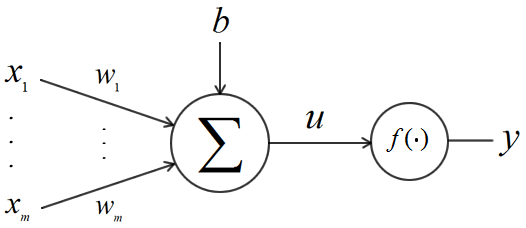
\includegraphics[width=.5\textwidth]{figuras/perceptron.png}
\caption{Modelo do neurônio artificial perceptron. [Imagem: \href{ http://computacaointeligente.com.br}{ http://computacaointeligente.com.br}]}
\label{figperceptron}
\end{figure}

A função \(\theta\) é conhecida como função de ativação ou função de transferência. Dentre as funções de ativação mais utilizadas estão a sigmoide e a tangente hiperbólica, definidas pelas equações abaixo, respectivamente \cite{articlefunclogtan}:

\begin{equation} \label{eq2}
\begin{split}
\theta(u) & = \frac{1}{1+ e^{-au}}\\
\theta(u) & = \frac{e^u - e^{-u}}{e^u + e^{-u}}
\end{split}
\end{equation}

\subsection{Arquitetura de uma RNA}
\label{subsec:redes-neurais-artificiais:arquitetura}

A arquitetura de uma RNA está relacionada com a maneira pela qual os seus neurônios estão organizados. De acordo com \cite{furtado2019redes}, as arquiteturas das RNAs são subdivididas em 3 classes: Rede Neural Feedforward de 1 camada, Rede Neural Feedforward Multicamadas e Redes Recorrentes ou Realimentadas. Além disso, a rede também é dividida em três tipos de camadas: a de entrada, a escondida e a de saída. 


As camadas podem ser classificadas em camadas de entrada, onde os padrões são apresentados à rede; camadas ocultas, onde é feita a maior parte do processamento; e a camada de saída, onde a conclusão do processamento é apresentada \cite{furtado2019redes}. Normalmente uma rede neural possui uma camada de entrada, uma camada de saída e \(k\) camadas ocultas, no qual \(k\) é definido empiricamente e varia de acordo com o problema.

Redes neurais do tipo Feedforward são redes de múltiplas camadas, ou seja, elas tem \(k\) camadas ocultas, no qual, a informação propaga-se da entrada para a saída, no caso, os sinais provenientes dos neurônios de uma camada só podem estimular os neurônios da camada seguinte. Quando a rede possuir todos os nós de uma camada comunicando-se com todos os nós da camada posterior, ela é dita totalmente conectada. Caso alguma das conexões sinápticas não esteja ligada com a camada subsequente, a rede é dita parcialmente conectada \cite{furtado2019redes}. A Figura \ref{figredeFeedforwardMulticamada} representa uma rede Feedforward multicamada de uma camada oculta totalmente conectada, ou seja, $k=1$.

% \begin{figure}[h]
% \centering
% 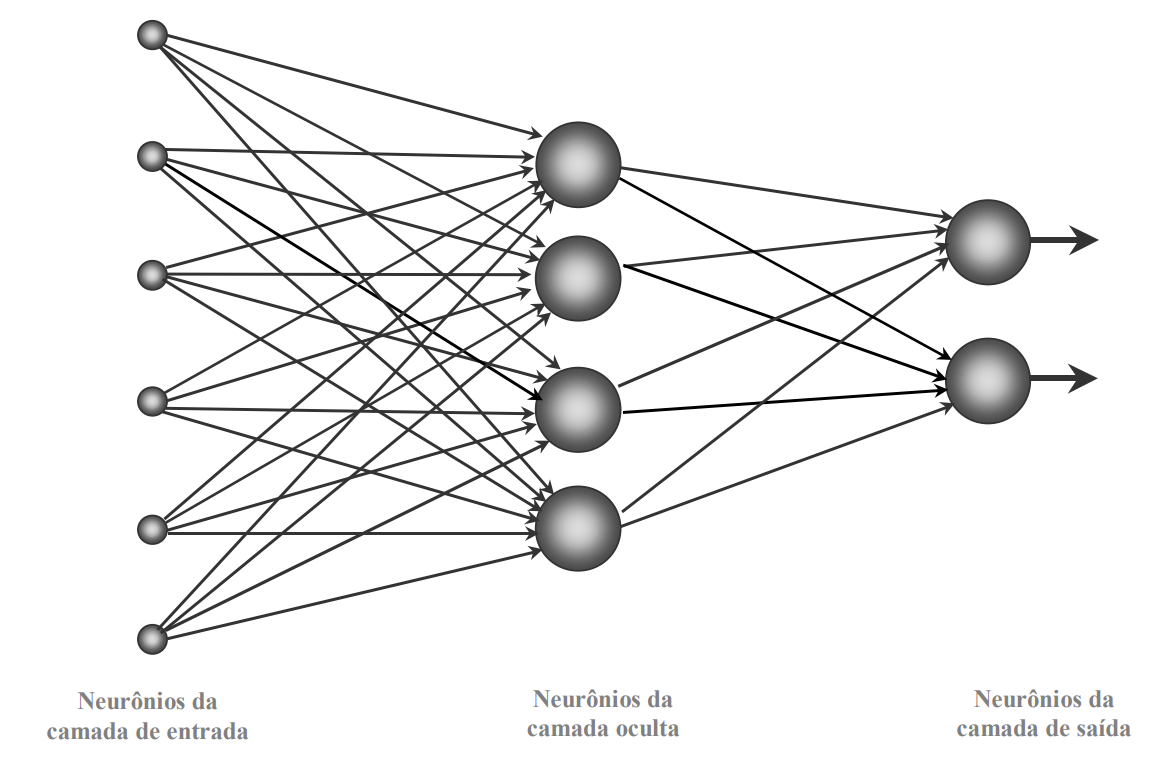
\includegraphics[width=.75\textwidth]{figuras/multicamadas.png}
% \caption{Exemplo de rede neural artificial do tipo Feedforward multicamadas. [Imagem: \cite{furtado2019redes}]}
% \label{figredeFeedforwardMulticamada}
% \end{figure}

\begin{figure}[h]
\centering
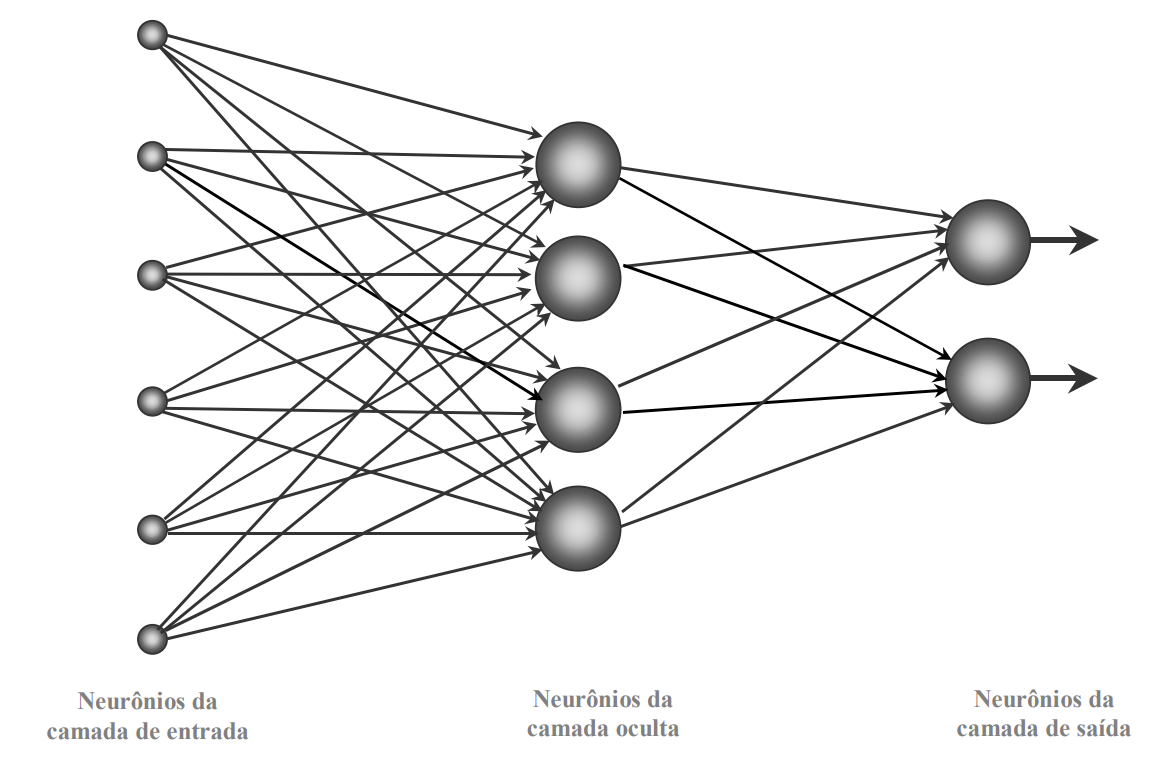
\includegraphics[width=.75\textwidth]{figuras/multicamadas.png}
\caption{Exemplo de rede neural artificial do tipo Feedforward multicamadas. [Imagem: \cite{furtado2019redes}]}
\label{figredeFeedforwardMulticamada}
\end{figure}

\subsection{Algoritmo de Treinamento}
\label{subsec:redes-neurais-artificiais:algoritmo}

A arquitetura da rede define, dentre outros parâmetros, a que tipo de treinamento a rede será submetida, capacitando-a a resolver o problema. No processo de treinamento a rede ‘aprende’ através de exemplos que relacionam as entradas e saídas do problema a ser solucionado. Essa abordagem é conhecida como aprendizado supervisionado. Dentre os algoritmos conhecidos, para solucionar esse tipo de problema, o mais utilizado é o backpropagation \cite{rumelhart1986learning}. A ideia do algoritmo é estimar os valores dos pesos e bias minimizando o erro entre a entrada e a saída desejada. O erro \(E\) cometido pela rede é calculado por:

\begin{equation} \label{eq3}
\begin{split}
E = \frac{1}{2} \sum_{i=1}^{p} \sum_{j=1}^{n} (d_{j}^{i} - y_{j}^{i})^2
\end{split}
\end{equation}
no qual, \(p\) é o número exemplos a ser utilizados no treinamento, n é o número de saídas da rede e, finalmente, \(d\) e \(y\) são as saídas desejadas e obtidas, respectivamente, para a entrada em questão.

Se o erro \(E\) encontrado for retropropagado (termo que foi derivado do nome do algoritmo backpropagation) pela rede, isto é, se o erro for propagado a partir da camada de saída até a camada de entrada, ela tentará estabelecer o quanto cada sinapse contribuiu para o erro, e este será usado para ajustá-las. A regra de atualização de cada peso sináptico da rede é calculado pela seguinte equação:

\begin{equation} \label{eqRNA4}
\begin{split}
W = W + \Delta W \therefore \Delta W = - \alpha\frac{\partial E}{\partial W}
\end{split}
\end{equation}

onde, \(\alpha\) é conhecido como taxa de aprendizado, que, resumidamente, indica o ‘tamanho do passo’ do gradiente rumo a minimização. O sinal negativo indica a busca por uma alteração no peso que reduza \(E\), sendo assim, quanto menor o erro, melhor a rede estará mapeando o problema.